\documentclass[10pt]{beamer}

\usetheme[progressbar=frametitle]{metropolis}
\usepackage{appendixnumberbeamer}

\usepackage{booktabs}
\usepackage[scale=2]{ccicons}

\usepackage{pgfplots}
\usepgfplotslibrary{dateplot}
\usepackage[portuguese]{babel}
\usepackage{amsmath}
\usepackage{bm}


\usepackage{xspace}
\newcommand{\themename}{\textbf{\textsc{metropolis}}\xspace}

\title{Exame de qualificação de mestrado}
\subtitle{Aprendizagem de representação através do uso de redes neurais convolucionais na recuperação de trecho de código-fonte}
% \date{\today}
\date{}
\author{Marcelo de Rezende Martins\\{\footnotesize sob orientação do Prof. Dr. Marco Aurélio Gerosa}}
\institute{Instituto de Pesquisas Tecnológicas do Estado de São Paulo - IPT}
% \titlegraphic{\hfill\includegraphics[height=1.5cm]{logo.pdf}}

\begin{document}

\maketitle

\begin{frame}{Índice}
  \setbeamertemplate{section in toc}[sections numbered]
  \tableofcontents%[hideallsubsections]
\end{frame}

\section[Intro]{Introdução}


\begin{frame}[fragile]{Definição}

\begin{quote}
Recuperação de trecho de código-fonte consiste em recuperar um trecho de código a partir de um repositório de códigos-fontes, de modo a atender a intenção do desenvolvedor, expressa em linguagem natural \cite{cambronero-deep-learning-code-search:2019, Gu-deep-code-search:2018}.     
\end{quote}


\end{frame}
\begin{frame}[fragile]{Definição (ERRATA)}

  \textbf{Code Retrieval}: Dada uma questão em linguagem natural $q \in \mathbb{Q}$, um modelo $F_{r}$ será treinado a recuperar os trechos $\mathbb{C}^{+} \subset \mathbb{C}_{a}$ com a maior pontuação:

\begin{equation}\label{eq:code-retrieval}
\mathbb{C}^{+} = \underset{c \in \mathbb{C}_{a}}{argmax}\text{ } F_{r}(q , c)
\end{equation}
\end{frame}


\section{Abordagem}

\begin{frame}{Joint Embedding}
    Sejam $\mathbb{Q}$ e $\mathbb{C}$ conjuntos de dados heterogêneos. \textit{Joint embedding} pode ser formulado como:
	\begin{equation}
        f: q \rightarrow t_{q} \rightarrow h_{\theta}(t_{q}, t_{c}) \leftarrow t_{c} \leftarrow c :g
    \end{equation}
\end{frame}

\begin{frame}{Joint Embedding}
   \begin{center}
       \begin{tabular}{|p{4cm}|p{4cm}|}
            \hline
            Como representar as palavras e os tokens das questões e trechos de código-fonte? & \textit{Word2Vec} \\ 
            \hline
            Como representar as sentenças? &  CNN \\
            \hline
            Como aproximá-los? &  Função de custo \textit{hinge} \\
            \hline
       \end{tabular}
   \end{center}
\end{frame}

\begin{frame}{Arquitetura}
	\begin{figure}[h]
        \centering
        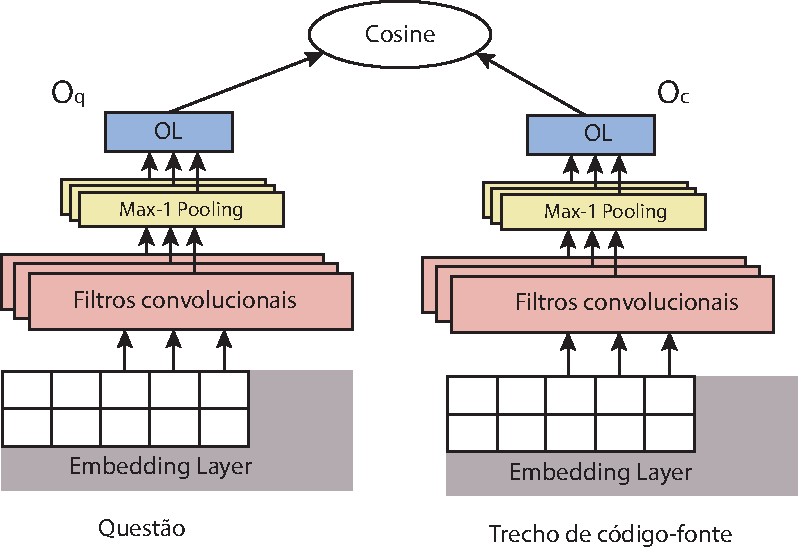
\includegraphics[width=0.8\linewidth]{figuras/cnn-architecture-proposal.pdf}
        \caption{Arquitetura CNN proposta para recuperação de trecho de código-fonte.}
        \label{fig:cnn-architecture-proposal}
    \end{figure}
\end{frame}


\begin{frame}{CNN}
	\begin{figure}[h]
        \centering
        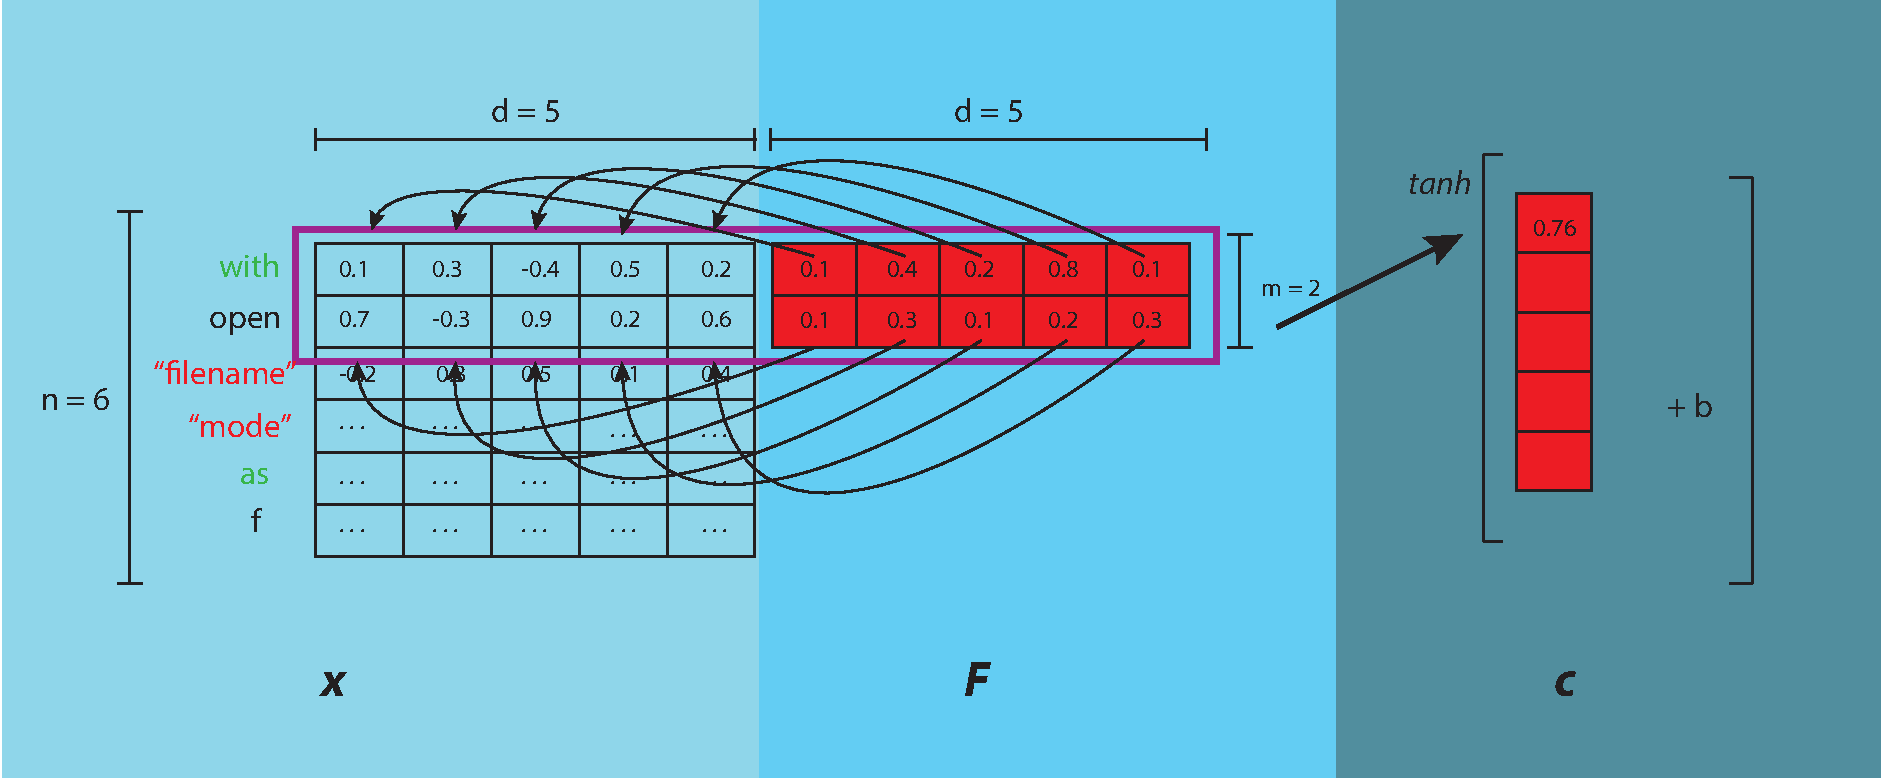
\includegraphics[width=1\linewidth]{figuras/first-step-convolution.pdf}
        \caption{Primeiro passo da operação de convolução em um vetor de entrada $\bm{x}$ composto por vetores de representação distribuída de cada palavra da sentença. }
        \label{fig:first-step-convolution}
    \end{figure}
\end{frame}

\section{Perguntas}


\begin{frame}{Perguntas}
	\begin{itemize}
	    \item A aprendizagem de representação através do CNN auxilia na recuperação de trecho de código-fonte?
	    \item O CNN é capaz de extrair as características mais relevantes de modo a facilitar o modelo a encontrar uma correlação entre as questões e os trechos de código-fonte?
	\end{itemize}
	Indiretamente:
	\begin{itemize}
	    \item As interações locais auxiliam na aproximação das intenções aos trechos de código?
	\end{itemize}
\end{frame}

\begin{frame}{Avaliação}
   \begin{center}
       \begin{tabular}{|p{4cm}|p{4cm}|}
            \hline
            Dados de treinamento & Conjunto de pares de questões e trechos de código-fonte em Pytrhon coletados do Stack Overflow por \cite{yao-2018} \\ 
            \hline
            Dados para avaliação final & Conjunto de dados anotados manualmente e disponibilizados por \cite{yao-2018} \\
            \hline
            Métrica de desempenho & \emph{MRR} \\
            \hline
            Arquiteturas de referência para comparação & \begin{itemize}
                \item Embedding
                \item Rede neural com mecanismo de atenção proposto por \cite{cambronero-deep-learning-code-search:2019}
            \end{itemize} \\
            \hline
       \end{tabular}
   \end{center}
\end{frame}

\begin{frame}{Avaliação}
   \begin{center}
       \begin{tabular}{|p{4cm}|p{4cm}|}
            \hline
            Análise dos resultados & \begin{itemize}
                \item Inspeção manual
                \item Análise dos piores casos
                \item Patologia das redes neurais \cite{feng-etal-2018-pathologies}
            \end{itemize} \\
            \hline
       \end{tabular}
   \end{center}
\end{frame}

\section{Experimento piloto}

\section{Próximos passos}



{\setbeamercolor{palette primary}{fg=black, bg=yellow}
\begin{frame}[standout]
  Questions?
\end{frame}
}

\appendix



\begin{frame}[allowframebreaks]{References}

  \bibliography{demo}
  \bibliographystyle{abbrv}

\end{frame}

\end{document}
